%! Suppress = MissingImport
%! Suppress = TooLargeSection
%! Suppress = SentenceEndWithCapital
%! Suppress = LineBreak
%! Suppress = MissingLabel
%! Suppress = Unicode

\documentclass[main.tex]{subfiles}

\begin{document}

    \section{Reprezentacja liczb całkowitych; arytmetyka.}

    \subsection{Kod znak-moduł prosty}
    \begin{itemize}
        \item \textbf{Reguły}:
        \begin{itemize}[noitemsep]
            \item Sygnalizacja znaku poprzez najwyższą pozycję,
            \item Cyfra 0 na pozycji znaku oznacza dodatniość,
            \item Brak kodowania cyfr wyrażajacych wartość.
        \end{itemize}
        \item \textbf{Przykład}: $q = 10, c = 5, u = 2, n = 8$
        \[[+216.7]_{zmp} = 0|00216.70, ~~ [-216.7]_{zmp} = 1|00216.70\]
        \item \textbf{Arytmetyka}: skomplikowana i czasochłonna, nie nadaje się do praktycznego stosowania.
    \end{itemize}

    \subsection{Kod odwrotnościowy}
    \begin{itemize}
        \item \textbf{Reguły}:
        \begin{itemize}[noitemsep]
            \item Najbardziej znacząca cyfra jest cyfrą znaku.
            \item Zerowa cyfra znaku oznacza dodatniość, najwyższa w systemie - ujemność
            \item Cyfry wartości dodatniej pozostają bez zmian
            \item Cyfry wartości ujemnej uzupełnione do najwyższej cyfry systemu
        \end{itemize}

        \item \textbf{Przykład}: q = 10, c = 7, u = 5
        \begin{gather*}
        [182073.6954]
            _{odw} = 0|0182073.69540\\
            [-182073.6954]_{odw} = [-0|0182073.69540]_{odw} = 9|9917926.30459
        \end{gather*}

        \item \textbf{Arytmetyka} -- sumowanie: dodaj kody, a w przypadku przepełnienia zwiększ wynik o najmniejszą
        możliwą liczbę dodatnią.
    \end{itemize}

    \subsection{Kod uzupełnieniowy}

    \begin{itemize}
        \item \textbf{Kodowanie} -- jak w odwrotnościowym, dla ujemnych z dodaniem 1 na najmniej znaczącym bicie.
        \item \textbf{Przykład}
        \begin{gather*}
        [182073.6954]
            _{uz} = 0|0182073.69540\\
            [-182073.6954]_{uz} = [-0|0182073.69540]_{odw} + [0|0000000.00001] = 9|9917926.30460
        \end{gather*}

        \item \textbf{Arytmetyka} -- suma kodów uzupełnieniowych jest zawsze kodem uzupełnieniowym sumy. Przepełnienie
        pomijamy.
    \end{itemize}

    \subsection{Kod nadmiarowy}
    \begin{itemize}
        \item \textbf{Kodowanie}
        \begin{itemize}[noitemsep]
            \item Liczba dodatnia ma niezerową cyfrę znaku.
            \item Kod nadmiarowy liczby ujemnej to kod uzupełnieniowy z 0 na pozycji znaku.
        \end{itemize}
        \item \textbf{Przykład}
        \begin{gather*}
        [182073.6954]
            _{nad} = 9|0182073.69540\\
            [-182073.6954]_{nad} = [9|9917926.30460] + [1|0000000.00000] = 0|9917926.30460
        \end{gather*}

        \item \textbf{Arytmetyka} -- suma kodów nadmiarowych to suma liczb z powiększonym o 1 znakiem (korekta: odjęcie
        1 od znaku).
    \end{itemize}


    \section{Reprezentacja liczb rzeczywistych; arytmetyka zmiennopozycyjna.}

    \subsection{Reprezentacja cecha-mantysa}
    Liczby postaci
    \[ m \times q^c \]

    \begin{itemize}[noitemsep]
        \item $q$ -- \textbf{podstawa} systemu liczbowego,
        \item $m$ - \textbf{mantysa} -- ciąg najbardziej znaczących cyfr liczby.
        \item $c$ - \textbf{cecha} -- wykładnik potęgi podstawy systemu
        \item W rejestrze komputera pamiętane są wyłącznie mantysa oraz cecha, zaś podstawa systemu jest ustalona, zatem nie musi być reprezentowana i nie jest konieczna do działań.
        \item Różnorodne sposoby zapamiętania w komputerze liczb w postaci cecha-mantysą noszą nazwę \textbf{kodowań zmiennopozycyjnych.}

    \end{itemize}

    \subsection{Kodowanie zmiennopozycyjne}
    \begin{itemize}[noitemsep]
        \item Powszechnie stosowane w komputerach dla reprezentacji \textbf{liczb rzeczywistych}.
        \item W systemie \textbf{dziesiętnym} dla oddzielenia mantysy i cechy powszechne użycie litery \textbf{E} (lub e), np.
        liczba $28.05 = 28.05e0 = 2805e-2 = 2.805e1$ itd.

        \item W systemie \textbf{binarnym} dla oddzielenia mantysy i cechy powszechne użycie litery \textbf{D} (lub d), np.
        liczba $1001.101 = 1001.101d0 = 1.001101d11$.

        \item Różnorodność reprezentacji wymusza konieczność ujednoznacznienia (\textbf{normalizacji}).

    \end{itemize}

    \subsection{Normalizacja}

    \begin{table}[H]
        \centering
        \begin{tabular}{l|l|l|l}
            & normalizacja
            całkowita & normalizacja
            do jedynki & normalizacja
            do ułamka  \\
            \hline
            28.05 & \texttt{2805e-2}                & \texttt{2.805e1}                  & \texttt{.2805e2}                  \\
            $(1001.101)_2$    & \texttt{1001101d-11}             & \texttt{1.001101d11}              & \texttt{.1001101d100}             \\
        \end{tabular}
    \end{table}

    \subsection{Algorytm kodowania zmiennopozycyjnego}
    \begin{itemize}[noitemsep]
        \item $w_m$ - liczba cyfr reprezentacji mantysy (bez cyfry znaku)
        \item $w_c$ - liczba cyfr reprezentacji cechy (bez cyfry znaku)
        \item n - liczba cyfr rejestru
    \end{itemize}
    \[ n = 1 + w_m + 1 + w_c \]

    \begin{enumerate}[noitemsep]
        \item Przedstaw liczbę w systemie o podstawie q.
        \item Zaokrąglij wartość liczby do $w_m$ cyfr.
        \item Zaokrąglony wynik sprowadź do znormalizowanej postaci
        potęgowej $m\cdot q^c$
        \item Jeżeli cecha jest zbyt duża (zbyt dodatnia) by zmieścić się
        w przewidzianym zakresie $w_c$ to zasygnalizuj błąd przepełnienia i zakończ.
        \item Jeżeli cecha jest zbyt mała (zbyt ujemna) by zmieścić się
        w zakresie $w_c$ to zakoduj zerową mantysę oraz zerową wartość cechy i zakończ.
        \item Zakoduj stałopozycyjnie mantysę na $w_m + 1$ pozycjach.
        \item Zakoduj stałopozycyjnie cechę na $w_c + 1$ pozycjach.
    \end{enumerate}

    \subsection{Arytmetyka}
    Brak ogólnego działania - dekodowanie i wykonywanie operacji wprost.

    \noindent \textbf{Dodawanie}:
    \begin{enumerate}[noitemsep]
        \item Zmodyfikuj mantysy dla zrównania cech.
        \item Wyznacz mantysę sumy w postaci sumy mantys.
        \item Zaokrąglij sumę mantys do liczby cyfr rejestru.
        \item Znormalizuj wynik.
    \end{enumerate}

    \noindent \textbf{Mnożenie}:
    \begin{enumerate}[noitemsep]
        \item Mantysa iloczynu to iloczyn mantys.
        \item Cecha iloczynu to suma cech.
        \item Zaokrąglij mantysę wyniku.
        \item Znormalizuj mantysę modyfikując cechę.
    \end{enumerate}


    \section{Różnice w wywołaniu funkcji statycznych, niestatycznych i wirtualnych w C++.}

    \subsection{Funkcje statyczne.}
    \begin{itemize}
        \item \textbf{Globalne funkcje statyczne} to funkcje o zakresie widoczności ograniczonym do
        ich \textit{jednostki translacji}, czyli pliku kompilowanego - pliku źródłowego z dołączonymi includami).
        \item \textbf{Metody statyczne klas} to metody których wywołanie jest niezależne od instancjonowania klasy -
        wszystkie instancje klasy współdzielą kopię statycznych metod i pól. Instancja nie jest nam potrzebna, ale
        można jej użyć.
    \end{itemize}

    \subsection{Funkcje niestatyczne.}
    \begin{itemize}
        \item \textbf{Niestatyczne funkcje globalne} są dostępne ze wszystkich plików, które includują zawierające
        je plik źródłowy - trzeba zatem uważać na konflikty nazw.
        \item \textbf{Nietstatyczne metody klas} wymagają do wywołania instancji klasy - mogą zachowywać się różnie
        dla różnych instancji; mogą być oznaczone \texttt{final} i \texttt{override}.
    \end{itemize}

    \subsection{Funkcje wirtualne.}
    \begin{itemize}
        \item \textbf{Wirtualne metody klas} są przydatne w polimorfiźmie.
        \item W przypadku zwykłej metody, wywołanie jej dla wskaźnika typu klasy podstawowej zawsze wywoła instancję
        z klasy podstawowej, nawet jeżeli wskaźnik będzie tak naprawdę wskazywał na klasę pochodną.
        \item Słowo kluczowe \texttt{virtual} \textbf{wymusza dedukcję} której metody użyć \textbf{na podstawie zawartości
        \item wskaźnika}, a \textbf{nie} jego \textbf{typu}. Dedukcja następuje w czasie wykonania programu.
    \end{itemize}


    \section{Sposoby przekazywania parametrów do funkcji (przez wartość, przez referencję). Zalety i wady.}

    \subsection{Przekazywanie przez wartość.}

    Przekazywanie argumentu przez wartość oznacza, że argumentem może być \textbf{rvalue} (np. wyrażenie arytmetyczne), a przekazanie
    \textbf{lvalue (zmiennej)} powoduje utworzenie \textbf{kopii}.
    \begin{itemize}
        \item Zaletą jest \textbf{możliwość użycia wyrażenia} w wywołaniu,
        \item \textbf{Tworzenie kopii} może być zaletą lub wadą - umożliwia nam to swobodne modyfikowanie wartości
        bez modyfikowania oryginalnej zmiennej, ale może stanowić niepotrzebne obciążenie pamięciowe.
    \end{itemize}

    \subsection{Przekazywanie przez referencję.}
    Funkcja otrzymuje jako argument \textbf{adres} zmiennej, a \textbf{nie} jej \textbf{wartość}. Wszelka modyfikacja takiego argumentu wewnątrz funkcji powoduje zmianę skojarzonej
    z tym argumentem zmiennej.
    \begin{itemize}
        \item Zaletą jest \textbf{nietworzenie niepotrzebnych kopii}, możliwość zmiany zmiennej spoza zakresu funkcji (zamiast
        np. zwracania i przypisywania nowej wartości).
        \item Nieprzemyślane użycie może spowodować \textbf{nieprzewidzianą} przez programistę \textbf{zmianę zawartości} zmiennej.
        \item \textbf{Brak możliwości użyca wyrażenia} jako argumentu funkcji - musimy zapisać jego wynik w zmiennej, by móc
        ją przekazać.
    \end{itemize}


    \section{Wskaźniki, arytmetyka wskaźników, różnica między wskaźnikiem a referencją w C++.}
    \textbf{Wskaźnik} – typ zmiennej odpowiedzialnej za przechowywanie \textbf{adresu} do innej zmiennej
    (innego miejsca w pamięci) w obrębie naszej aplikacji.
    Wskaźnik może wskazywać na jakąś zmienną, strukturę, tablicę czy nawet funkcję.

    \noindent\textbf{Operatory związane ze wskaźnikami w C++}

    \begin{itemize}[noitemsep]
        \item \texttt{int * intPtr} -- wskaźnik na int
        \item \texttt{intPtr = \&a} -- ampersand jako pobranie adresu
        \item \texttt{cout << *intPtr} -- dereferencja
    \end{itemize}

    \noindent \textbf{Arytmetyka wskaźników} --
    mając wskaźnik \texttt{int *p} wskazujący na hipotetyczny adres 10, wykonując na nim operację \texttt{p+2}
    dostajemy wskaźnik wskazujący na adres \texttt{10 + 2*sizeof(int)}.
    Jest to przydatne szczególnie przy operowaniu na strukturach, których pola są ułożone po kolei w pamięci, np. tablicach
    (\texttt{*(a+i) $=$ \texttt[a[i]]}).\\


    \noindent \textbf{Referencja} -- można ją traktować jako dodatkową nazwę na już istniejący obiekt, coś w rodzaju
    stałego wskaźnika. Składnia referencji \textbf{zabrania wykonywania operacji wskaźnikowych} -- \textbf{nie można
    zmienić} referowanego \textbf{obiektu}.
    \begin{itemize}
        \item Łatwiejsza notacja - nie musimy używać operatora wyłuskania (\texttt{*}) do odwoływania się do obiektu -
        odwołanie do referencji powoduje odwołanie do obiektu.
        \item Większe bezpieczeństwo - brak arytmetyki dla referencji znacznie utrudnia popełnienie błędów związanych
        z niepoprawnym odwołaniem do pamięci.
    \end{itemize}

    \noindent \textbf{Po kompilacji} (w kodzie maszynowym) referencje i wskaźniki \textbf{nie różnią się}.


    \section{Podstawowe założenia paradygmatu obiektowego: dziedziczenie, abstrakcja, enkapsulacja, polimorfizm.}

    \textbf{Dziedziczenie (kompozycja)}:
    \begin{itemize}[noitemsep]
        \item Umożliwia stworzenie \textbf{hierarchii obiektów} w programie.
        \item Polega na \textbf{przejęciu} właściwości i \textbf{funkcjonalności} obiektów klasy bazowej
        i \textbf{ewentualnej} ich \textbf{modyfikacji}.
        \item Np. dziedziczenie klasy "Kot" po klasie "Zwierzę" i nadpisanie wirtualnej metody "dajGłos".
    \end{itemize}


    \noindent \textbf{Abstrakcja}:
    \begin{itemize}[noitemsep]
        \item Dany obiekt w systemie służy jako \textbf{model abstrakcyjnego "wykonawcy"}, który może wykonywać pracę, opisywać i zmieniać swój stan, oraz komunikować się
        z innymi obiektami w systemie, bez ujawniania, w jaki sposób zaimplementowano dane cechy.
        \item Uogólnienie pewnego zbioru problemów do wspólnego zbioru zachowań i cech \textbf{niezależnych od implementacji}.
    \end{itemize}

    \noindent \textbf{Enkapsulacja} (hermetyzacja, kapsułkowanie):
    \begin{itemize}[noitemsep]
        \item \textbf{Ukrywanie pewnych danych} składowych lub metod obiektów danej klasy tak, aby były one
        \textbf{dostępne} tylko \textbf{metodom wewnętrznym} danej klasy lub funkcjom zaprzyjaźnionym, nie bezpośrednio.
        \item Zapewnia, że obiekt nie może zmieniać stanu innych obiektów w nieokreślony sposób; dostarcza interfejsu,
        który określa sposób współpracy z innymi obiektami.
        \item Gettery, settery i funkcje zaprzyjaźnione.
    \end{itemize}

    \noindent \textbf{Polimorfizm} (wielopostaciowość):
    \begin{itemize}[noitemsep]
        \item \textbf{Referencje i wskaźniki obiektów mogą dotyczyć obiektów różnego typu}.
        \item Dla obiektu zapisanego w pointerze na klasę bazową -- domyślnie dedukcja wartości z klasy bazowej, przy
        wirtualnych metodach - z faktycznego typu obiektu.
        \item Dwa rodzaje polimorfizmu: \textbf{dynamiczny} - wykonywany podczas działania programu, oraz
        \textbf{statyczny} - na etapie kompilacji.
    \end{itemize}


    \section{Funkcje zaprzyjaźnione i ich związek z przeładowaniem operatorów w C++.}
    \begin{itemize}
        \item \textbf{Funkcja zaprzyjaźniona} dla danej klasy to funkcja oznaczona \textbf{słowem kluczowym
        \textit{friend}}.
        \item Funkcja ta ma \textbf{dostęp do niepublicznych} (\textit{private} i
        \textit{protected}) \textbf{składowych} klasy.

        \item Mechanizm zaprzyjaźnienia jest specyficzny dla języka C++
        \begin{itemize}[noitemsep]
            \item Funkcje zaprzyjaźnione mogą się odnosić wyłącznie do \textbf{obiektów globalnych} lub danych przez
            argumenty
            \item \textbf{Dowolna ilość klas} może deklarować zaprzyjaźnienie jednej funkcji
            \item Funkcje zaprzyjaźnione mogą być \textbf{przeładowane}, zarówno w definiowanej klasie, jak i na zewnątrz
            \item Funkcje zaprzyjaźnione mogą być \textbf{definiowane wewnątrz klasy}, ale nie stanowią jej metody a
            szczególną definicję zewnętrznej funkcji.
        \end{itemize}

        \item Przy \textbf{przeładowaniu operatorów} często stosuje się \textbf{\textit{friend}}  w celu dostępu do pól
        prywatnych przez funkcje zewnętrzne (np. dla operatora \texttt{<<}).
    \end{itemize}


    \section{Programowanie generyczne na podstawie szablonów w języku C++.}

    To \textbf{paradygmat programowania} w którym algorytmy (funkcje, klasy) są zapisywane \textbf{bez specyfikacji typów},
    na których działają.
    W C++ szablony \textbf{\textit{template}} pozwalają na programowanie generyczne.\\

    \noindent \textbf{Zalety} szablonów:
    \begin{itemize}[noitemsep]
        \item Zmniejszają redundancję
        \item Wydajny, elastyczny, wielozadaniowy kod (STL)
        \item Metaprogramowanie
        \item Polimorfizm rozwiązywany w czasie kompilacji
    \end{itemize}

    \noindent    W C++ istnieją szablony klas, struktur, funkcji (również metod), szablonów.
    \begin{itemize}[noitemsep]
        \item Argumenty końcowe szablonu mogą mieć wartości domyślne.
        \item Możliwość \textbf{specjalizacji szablonu} -- dostarczenia niestandardowego kodu dla danego zestawu
        argumentów -- np. \textbf{vector booli} przechowywany na bitach.
    \end{itemize}


    \section{Podstawowe kontenery w STL z szerszym omówieniem jednego z nich.}
    \textbf{Standard Template Library} (STL) to biblioteka C++ zawierająca algorytmy, kontenery, iteratory oraz inne
    konstrukcje w formie szablonów, gotowe do użycia w programach.\\

    \noindent Kontenery zarządzają \textbf{pamięcią alokowaną} do przechowywania ich elementów, i zapewniają metody
    pozwalające na dostęp do nich, bezpośrednio lub przez iteratory (obiekty o właściwościach podobnych do wskaźników).\\

    \noindent \textbf{Cztery rodzaje kontenerów}:
    \begin{itemize}[noitemsep]
        \item \textbf{Kontenery sekwencyjne} -- sekwencyjny dostęp do elementów struktury.
        \begin{itemize}
            \item array, vector, deque, forward\_list, list
        \end{itemize}

        \item \textbf{Adaptery} - kontenery wykorzystujące inny kontener zapewniając mu pożądanych interfejs,
        np. \texttt{stack} oferujący działania stosu dla np. wektora.
        \begin{itemize}
            \item stack, queue, priority\_queue
        \end{itemize}

        \item \textbf{Kontenery asocjacyjne} -- implementują posortowane struktury danych, które da się szybko
        przeszukiwać (złożoność O(log n))
        \begin{itemize}
            \item set, multiset, map, multimap
        \end{itemize}

        \item \textbf{Nieuporządkowane kontenery asocjacyjne} -- implementują nieposortowane (haszowane)
        struktury danych, które mogą być szybko przeszukiwane (zamortyzowana złożoność O(1), w najgorszym przypadku O(n))
        \begin{itemize}
            \item unordered\_set, unordered\_multiset, unordered\_map, unordered\_multimap
        \end{itemize}
    \end{itemize}

    \noindent Przykładowy kontener: \textbf{\texttt{std::array}}:
    \begin{itemize}[noitemsep]
        \item wyraża tablicę o \textbf{stałej ilości} elementów, ustalonejw czasie kompilacji przez argument
        \textbf{templatki},
        \item dostęp \textbf{sekwencyjny} do elemenów -- pewien ustalony porządek,
        \item \textbf{statyczny przydział pamięci} -- nie mogą zmienić rozmiaru,
        \item mogą być traktowane jako \textbf{krotki},
        \item swap dwóch tablic wymaga ich przepisania w czasie liniowym -- za to iteratory odnoszą się ciągle
        do tych samych adresów
    \end{itemize}


    \section{Obsługa sytuacji wyjątkowych w C++.}
    \begin{itemize}
        \item Wyjątek = \textbf{obiekt sytuacji wyjątkowej}.
        \item Wyjątki pozwalają zareagować na \textbf{nieoczekiwaną sytuacje}, w której istnieje \textbf{ryzyko
        niewykonania} określonego \textbf{zadania}.
        \item Dawniej polegało to na zwróceniu specyficznej wartości, co wymuszało typ wyjątku (jako typ zwracany przez funkcję).
        \item W C++ wyjątki się "\textbf{rzuca}", służy do tego instrukcja \texttt{throw}. Rzucić możemy \textbf{błąd}
        (exception, error), ale też \textbf{typy} proste (int, char, string, \ldots) i \textbf{obiekty} klas.
        \item Tam gdzie spodziewamy się wyjątków umieszczamy bloki \textbf{\texttt{try-catch}}. Catche rozpatrywane są
        od góry.
    \end{itemize}


    \section{Obsługa plików w języku C.}

    Standardowa biblioteka wejścia/wyjścia języka C udostępnia funkcje do operowania na plikach, tj.
    odczytu i zapisu danych z plików tekstowych i binarnych (stdio.h, stdlib.h).

    \begin{enumerate}
        \item Otwarcie pliku o określonej nazwie w określonym trybie.
        \begin{minted}{cpp}
            FILE *fopen(const char *filename, const char *mode);
        \end{minted}
        Dostępne tryby (możliwość łączenia):
        \begin{itemize}[noitemsep]
            \item "r" - czytanie, "+" dodaje opcję nadpisywania,
            \item "w" - nadpisywanie, "+" dodaje odczyt,
            \item "a" - dopisywanie (ew. tworzenie), "+" dodaje odczyt,
            \item "t" - tryb tekstowy,
            \item "b" - tryb binarny.
        \end{itemize}
        Funkcja zwraca wskaźnik do pliku (FILE *) lub NULL, gdy pliku nie udało się otworzyć (nie
        istnieje, jest już otwarty w innym programie itp.).
        \textbf{Po zakończeniu pracy należy plik zamknąć} -- funkcja \texttt{fclose(file)}.

        \item Wykonywanie operacji odczytu/zapisu z możliwością formatowania.
        \begin{minted}{cpp}
            int fscanf(FILE *stream, const char *format, ...);
            int fprintf(FILE *stream, const char *format, ...);
        \end{minted}
        Funkcje działają tak jak scanf i printf, przy czym jako pierwszy argument przyjmują
        wskaźnik do pliku (strumienia danych).

    \end{enumerate}


    \section{Model wodospadu a model spiralny wytwarzania oprogramowania.}

    \subsection{Model kaskadowy}

    \textbf{Zasady}
    \begin{itemize}[noitemsep]
        \item Tworzenie systemu \textbf{sekwencyjnie, w wyizolowanych etapach};
        \item Wyjścia z jednego etapu są wykorzystywane jako wejścia do etapu następnego;
        \item Każdy etap podzielony jest na \textbf{dwie części}: \textbf{twórczą} i \textbf{weryfikacji};
        \item Ponowna praca, jeśli jest konieczna, jest wykonywana w kolejnych etapach -- bardzo \textbf{wysoki koszt błędów}
        popełnionych \textbf{we wstępnych etapach}, adaptowanie zmian bardzo kosztowne.
        \item Koszty opracowania i akceptacji dokumentów są wysokie, powinien być używany
        tylko jeśli wymagania są jasne i zrozumiałe; jakość silnie związana z ich stabilnością.
        \item \textbf{Marginalizacja roli klienta} w procesie wytwarzania oprogramowania. Uzyskanie produktu zgodnego z wymaganiami
        silnie zależne od ich stabilności.
    \end{itemize}

    \noindent \textbf{Fazy modelu kaskadowego}
    \begin{enumerate}
        \item \textbf{Planowanie}: cele biznesowe, podstawowe wymagania, założenia, standardy, parametry,
        \item \textbf{Analiza}: zdefiniowanie przeznaczenia systemu $\rightarrow$ kompletny, spójny i jednoznaczny model systemu,
        \item \textbf{Projekt}: dekompozycja na podsystemy, wybór strategii budowania, projektowanie obiektów, wybór komponentów, opis interfejsów,
        \item \textbf{Implementacja}: tworzenie kodu źródłowego, mapowanie modeli na kod,
        \item \textbf{Testowanie}: znajdowanie różnic między rzeczywistym elementem a jego modelem,
        \item \textbf{Pielęgnacja}.
    \end{enumerate}

    \subsection{Model spiralny}
    \begin{itemize}
        \item proces ma postać spirali, której każda pętla reprezentuje jedną jego fazę;
        \item najbardziej wewnętrzna pętla przedstawia początkowe etapy;
        \item ciągłe monitorowanie i pomiar zmian;
        \item zmiany poddawane są review użytkownika;
        \item próba minimalizacji ryzyka niepowodzenia;
    \end{itemize}

    \subsubsection{Fazy modelu spiralnego}
    Każda pętla spirali podzielona jest na cztery sektory
    \begin{enumerate}
        \item \textbf{Ustalanie celów} -– definiowanie konkretnych celów wymaganych w tej fazie przedsięwzięcia;
        identyfikacja ograniczeń i zagrożeń; ustalanie planów realizacji.
        \item \textbf{Rozpoznanie i redukcja zagrożeń} -– przeprowadzenie szczegółowej analizy rozpoznanych zagrożeń,
        ich źródeł i sposobów zapobiegania; podjęcie kroków zapobiegawczych.
        \item \textbf{Tworzenie i zatwierdzanie} –- tworzenie oprogramowania w oparciu o najbardziej odpowiedni model,
        wybrany na podstawie oceny zagrożeń.
        \item \textbf{Ocena i planowanie} –- recenzja postępu prac i planowanie kolejnej fazy przedsięwzięcia bądź
        zakończenie procesu produkcyjnego.
    \end{enumerate}


    \begin{table}[H]
        \centering
        \begin{tabular}{|p{4.8cm}||p{5.5cm}|p{5.5cm}|}
            \hline
            &\textbf{Model kaskadowy} & \textbf{Model spiralny}\\
            \hline
            \hline
            sposób działania & sekwencyjny & ewolucyjny\\
            \hline
            błędy & wykrywane i naprawiane po zakończeniu etapów & wykrywane wcześniej\\
            \hline
            rozmiar projektu & mniejsze & większe\\
            \hline
            wymagania & określone na początku & mogą być dodawane po iteracjach\\
            \hline
            zmiany w czasie projektu & ograniczona możliwość zmian & większa możliwość zmian\\
            \hline
            koszt & mały & wysoki\\
            \hline
        \end{tabular}
    \end{table}


    \section{Diagram sekwencji i diagram przypadków użycia w języku UML.}\label{sec:uml}

    \textbf{UML} - Unified Modelling Language.
    \begin{itemize}[noitemsep]
        \item \textbf{rodzina notacji graficznych};
        \item służy do \textbf{opisywania i projektowania} systemów informatycznych;
        \item narodził się z unifikacji wielu obiektowych języków modelowania graficznego;
        \item nadzorowany przez organizacje OMG.
    \end{itemize}

    \subsection{Diagram sekwencji.}

    \textbf{Diagram sekwencji} opisuje \textbf{interakcje pomiędzy częściami systemu} w postaci sekwencji
    komunikatów wymienianych między nimi.\\

    \noindent Diagramy sekwencji dobrze ukazują \textbf{dynamiczne aspekty realizacji scenariuszy}, w których dochodzi do złożonych
    oddziaływań pomiędzy obiektami.
    \begin{itemize}[noitemsep]
        \item \textbf{strzałka zwykła} -- przesłanie komunikatu asynchronicznego,
        \item \textbf{strzałka z wypełnionym grotem} -- wywołanie funkcji,
        \item \textbf{strzałka rysowana linią przerywaną} -- powrót z funkcji.
    \end{itemize}

    \begin{figure}[H]
        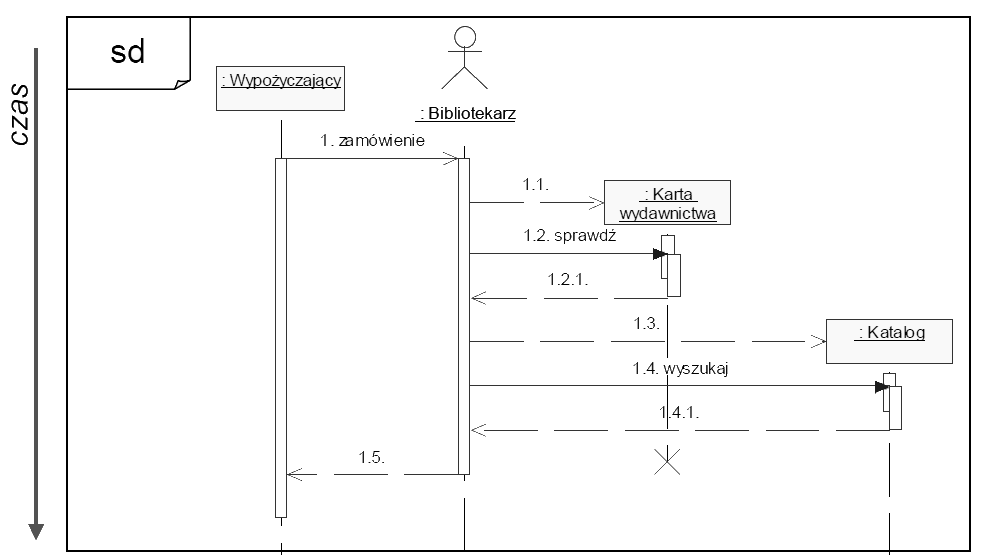
\includegraphics[width=\linewidth]{uml_sek.png}
    \end{figure}

    \subsection{Diagram przypadków użycia.}

    \textbf{Diagram przypadków użycia} służy do przedstawiania:
    \begin{itemize}[noitemsep]
        \item \textbf{interakcji aktora} z systemem,
        \item \textbf{zadań}, jakie wykonuje system,
        \item \textbf{wymagań} funkcjonalnych.
    \end{itemize}

    \noindent \textbf{Aktorami} mogą być ludzie, systemy zewnętrzne bądź części systemu, które mają wpływ na jego funkcjonowanie,
    ale są przezeń niezmienialne (np. zegar systemowy).

    \begin{figure}[H]
        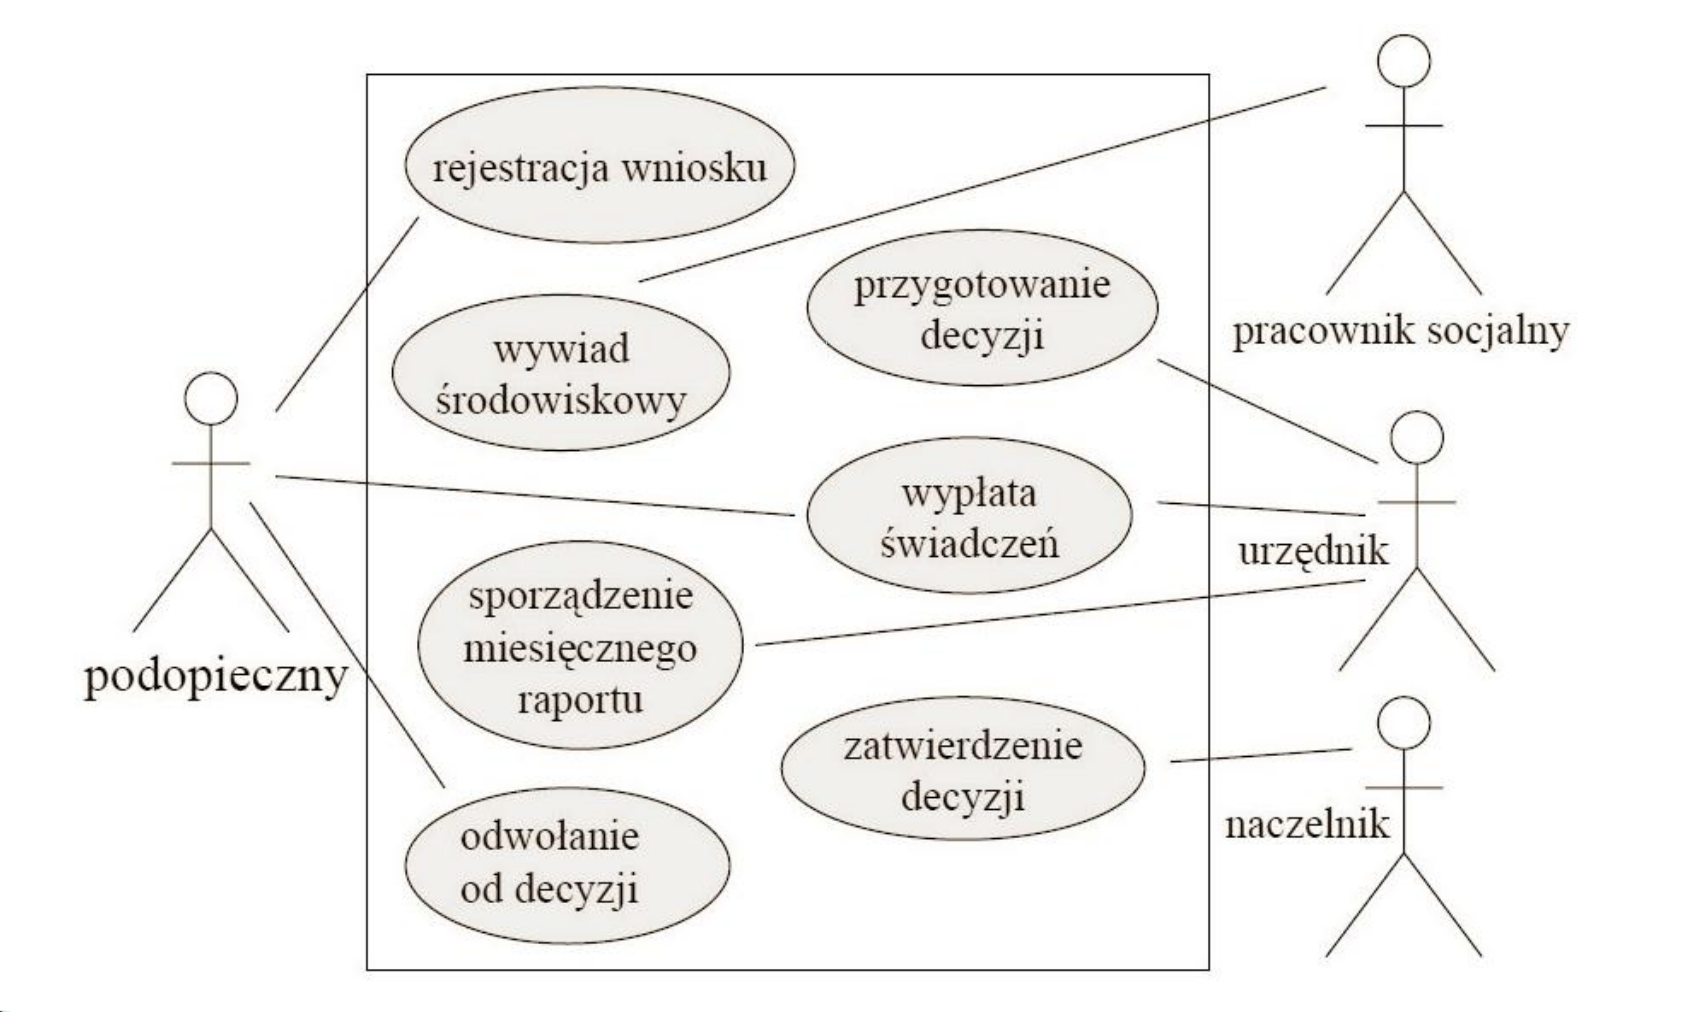
\includegraphics[width=\linewidth]{uml_pu.png}
    \end{figure}


    \section{Klasyfikacja testów.}

    \subsection{Poziomy testów.}
    \begin{definition}
        \textbf{Poziom testów} określa \textbf{sposób} testowania ze względu na \textbf{postać}
        testowanego obiektu w kontekście cyklu życia (\textbf{co testujemy?}).
    \end{definition}

    \begin{table}[H]
        \begin{center}
            \begin{tabular}{| p{4cm}| p{12cm}|}
                \hline
                \multicolumn{2}{|c|}{ \textbf{TESTY JEDNOSTKOWE}}\\
                \hline
                \textbf{Podstawa testów} & wymagania na moduły, projekt szczegółowy, kod\\
                \hline
                \textbf{Typowe obiekty} & moduły, programy, funkcje, klasy, procedury\\
                \hline
            \end{tabular}
        \end{center}
    \end{table}

    \begin{itemize}[noitemsep]
        \item testowanie modułowe, \textbf{unit testing} -- przeprowadzane przez \textbf{deweloperów}
        \item defekty szukane w izolacji od reszty systemu
        \item brak formalnego procesu zarządzania defektami; defekty \textbf{usuwane bezpośrednio po znalezieniu}
        \item wykorzystanie zaślepek i sterowników
        \item \textbf{TTD} -- Test Driven Developement -- napisanie testu, uruchomienie testu, napisanie kodu.
    \end{itemize}


    \begin{table}[H]
        \begin{center}
            \begin{tabular}{| p{4cm}| p{12cm}|}
                \hline
                \multicolumn{2}{|c|}{ \textbf{TESTY INTEGRACYJNE}}\\
                \hline
                \textbf{Podstawa testów} & projekt systemu, architektura, przypadki użycia\\
                \hline
                \textbf{Typowe obiekty} & interfejsy, podsystemy, konfiguracje systemów\\
                \hline
            \end{tabular}
        \end{center}
    \end{table}

    \begin{itemize}[noitemsep]
        \item testuje \textbf{interfejsy i interakcje}, wymaga \textbf{rozumienia architektury}
        \item może odbywać się na wielu poziomach (np. integracja systemów); im większy zakres integracji, tym trudniej izolować defekty,
        \item \textbf{strategie} testów integracyjnych:
        \begin{itemize}[noitemsep]
            \item \textbf{top-down} -- najpierw moduł wywołujący, potem wywoływane,
            \item \textbf{bottom-up} -- najpierw moduły wywoływany, potem wywołujący,
            \item \textbf{funkcjonalne} -- top-down wewnątrz danej funkcjonalności,
            \item \textbf{sekwencyja} przeprowadzania \textbf{transakcji},
            \item \textbf{big-bang} -- wszystko integrowane i testowane naraz.
        \end{itemize}
    \end{itemize}

    \begin{table}[H]
        \begin{center}
            \begin{tabular}{| p{4cm}| p{12cm}|}
                \hline
                \multicolumn{2}{|c|}{ \textbf{TESTY SYSTEMOWE}}\\
                \hline
                \textbf{Podstawa testów} & wymagania na system, przypadki użycia,
                specyfikacja funkcjonalna, raporty analizy ryzyka\\
                \hline
                \textbf{Typowe obiekty} & system, podręczniki użytkownika i operatora,
                konfiguracja systemu\\
                \hline
            \end{tabular}
        \end{center}
    \end{table}

    \begin{itemize}[noitemsep]
        \item sprawdza zachowanie \textbf{systemu jako całości} w środowisku testowym podobnym do \textbf{produkcyjnego},
        zwykle przez \textbf{niezależny zespół testerski}
        \item zakres testu określony w \textbf{planie testów}
        \item często konieczność testowania z \textbf{niekompletnymi wymaganiami}
    \end{itemize}


    \begin{table}[H]
        \begin{center}
            \begin{tabular}{| p{4cm}| p{12cm}|}
                \hline
                \multicolumn{2}{|c|}{ \textbf{TESTY AKCEPTACYJNE}}\\
                \hline
                \textbf{Podstawa testów} & wymagania użytkownika, wymagania na system,
                przypadki użycia, procesy biznesowe, raporty
                analizy ryzyka\\
                \hline
                \textbf{Typowe obiekty} & Procesy biznesowe w pełni zintegrowanego
                systemu, procesy operacyjne i utrzymania systemu,
                procedury, raporty, dane konfiguracyjne\\
                \hline
            \end{tabular}
        \end{center}
    \end{table}

    \begin{itemize}[noitemsep]
        \item cel: \textbf{uzyskanie zaufania} do systemu; często przeprowadzane przez klienta lub \textbf{użytkownika},
        \item znajdowanie defektów nie jest głównym celem
        \item \textbf{ocenia gotowość} systemu, ale niekoniecznie ostatni etap testów

        \item \textbf{typowe formy testów akceptacyjnych:}
        \begin{itemize}
            \item \textbf{testy akceptacyjne użytkownika (UAT)} – sprawdzenie gotowości do użycia
            \item \textbf{testy operacyjne (OAT)} – akceptacja przez administratora systemu (testy
            backupu, przywracania systemu, zarządzania użytkownikami itp.)
            \item \textbf{testy akceptacyjne wymagane kontraktem/regulacjami}
            \item \textbf{testy alfa, beta (polowe)}
            \begin{itemize}
                \item \textbf{alfa}: przeprowadzane \textbf{u producenta}, ale nie przez zespół
                \item \textbf{beta}: przeprowadzane \textbf{u klienta}, przez użytkownika
            \end{itemize}
        \end{itemize}
    \end{itemize}

    \subsection{Typy testów.}

    \begin{definition}
        \textbf{Typ testów} to zbiór czynności testowych właściwych dla weryfikacji systemu
        w oparciu o konkretny powód lub cel testów (\textbf{jak testujemy?}).
    \end{definition}

    \begin{enumerate}
        \item  \textbf{Testowanie funkcjonalne} -- testowanie funkcji -- \textbf{co system robi}.

        \item \textbf{Testowanie niefunkcjonalne} -- wyrażalne ilościowo testowanie niefunkcjonalnej charakterystyki
        jakościowej (np. niezawodność, wydajność, użyteczność) - \textbf{jak system działa}.

        \item \textbf{Testowanie strukturalne} -- oparte na strukturze (np. kod, graf przepływu sterowania, model procesu biznesowego).
        Zwykle wykonywane \textbf{po testach czarnoskrzynkowych}, aby ustalić \textbf{pokrycie}.

        \item \textbf{Retesty i testy regresji} -- \textbf{związane ze zmianą}, tzn. potwierdzenie usunięcia defektów
        (retesty - testy zmienionych fragmentów kodu) oraz poszukiwanie niezamierzonych zmian (regresyjne - testy
        niezmienionego kodu - często automatyzowane).
    \end{enumerate}


    \section{Model Scrum: struktura zespołu, proces wytwarzania oprogramowania, korzyści modelu.}
    \textbf{SCRUM} jest: lekki, łatwy do zrozumienia, bardzo trudny do opanowania.

    \noindent \textbf{Trzy filary} SCRUMu:
    \begin{itemize}[noitemsep]
        \item \textbf{Adaptacja} - powinna być \underline{ciągła}. Korekta musi być
        wykonana jak najszybciej, by ograniczyć dalsze następstwa problemów.
        \item \textbf{Przejrzystość} - wszystkie \underline{istotne aspekty} procesu
        muszą być \underline{widoczne} dla osób odpowiedzialnych za osiągane rezultaty.
        \item \textbf{Inspekcja} – poddawane \underline{regularnej} inspekcji są zarówno scrumowe
        artefakty jak i postępy prac.
    \end{itemize}

    \subsection{Role}:
    \begin{itemize}
        \item \textbf{Właściciel Produktu}
        \begin{itemize}[noitemsep]
            \item \textbf{odpowiedzialny} za maksymalizację wartości produktu i \textbf{pracy} Zespołu,
            \item jedyną osoba \textbf{zarządzająca Rejestrem} Produktu, tzn:
            \begin{itemize}[noitemsep]
                \item jasne artykułowanie \textbf{elementów}, określanie ich \textbf{kolejności};
                \item zapewnianie dostępności i przejrzystości dla wszystkich; opisywanie czym
                Zespół Scrumowy będzie się zajmował.
            \end{itemize}
        \end{itemize}

        \item \textbf{Zespoł deweloperski}
        \begin{itemize}[noitemsep]
            \item złożony z równych \textbf{profesjonalistów} -- "Deweloperów" (3-9 os); \textbf{samoorganizujący} się, wielofunkcyjny.
            \item ma za zadanie dostarczenie (na zakończenie każdego Sprintu), gotowego do wydania \textbf{Przyrostu}
            produktu,
            \item odpowiedzialność za wykonywaną pracę ponosi cały Zespół; \textbf{brak podziału na podzespoły}.
        \end{itemize}

        \item \textbf{Scrum Master} -- odpowiedzialny za to, by Scrum był rozumiany i stosowany, zarówno przez Właściciela,
        jak i Zespół.
    \end{itemize}

    \subsection{Zdarzenia}

    \begin{itemize}
        \item \textbf{Sprint} -- stałe przez okres trwania prac \textbf{ograniczenie czasowe} ($\leq$ 1 mies)
        \begin{itemize}[noitemsep]
            \item podczas Sprintu wytwarzany jest Przyrost funkcjonalności,
            \item niedozwolone są zmiany, które wpłyną na cel Sprintu,
            \item niezmienny skład Zespołu Deweloperskiego i jego cel jakościowy.
        \end{itemize}

        \item \textbf{Przerwanie Sprintu} -- przez Właściciela w przypadku dezaktualizacji celu Sprintu;
        zużywa zasoby, bo powoduje przegrupowanie podczas kolejnego Planowania.

        \item \textbf{Planowanie Sprintu} - 8h/mies
        \begin{itemize}[noitemsep]
            \item Część pierwsza: \textbf{Co będzie zrobione w tym Sprincie?}\\
            Na podstawie RP, ostatniego przyrostu i odczytów wydajności, oraz przewidywalnej pojemności ZD wyznacza się
            cel Sprintu i elementy RP do zrobienia.
            \item Część druga: \textbf{Jak wybrana praca będzie wykonana?}\\
            Stworzenie projektu systemu i planu prac; ZD powinien móc wytłumaczyć Właścicielowi i Scrum Masterowi,
            w jaki sposób ma zamiar pracować.
        \end{itemize}

        \item \textbf{Codzienny Scrum} - 15 min/d -- co zrobiłem od wczoraj, co chcę zrobić do jutra, co mi przeszkadzało.

        \item \textbf{Przegląd Sprintu} - 4h na zakończenie Sprintu
        \begin{itemize}[noitemsep]
            \item WP stwierdza, które funkcjonalności zostały „Ukończone”, a które nie;
            \item ZD omawia, co poszło dobrze, jakie były problemy i jak je rozwiązano;
            \item ZD prezentuje „Ukończoną” pracę i odpowiada na pytania;
            \item WP omawia RP w aktualnej jego postaci. Przewiduje termin zakończenia prac.
            \item Cała grupa omawia kolejne kroki.
        \end{itemize}

        \item \textbf{Retrospektywa Sprintu} - inspekcja działań i planowanie usprawnień.
        \begin{itemize}[noitemsep]
            \item co się działo, biorąc pod uwagę ludzi, zależności, procesy i narzędzia;
            \item Zidentyfikowanie i uporządkowanie istotnych elementów dobrych i złych,
            \item Stworzenie planu wprowadzania w życie usprawnień pracy Zespołu.
        \end{itemize}
    \end{itemize}

    \subsection{Artefakty}
    \begin{itemize}
        \item \textbf{Rejestr Produktu}
        \begin{itemize}[noitemsep]
            \item uporządkowana lista wszystkiego, co może być potrzebne w produkcie;
            \item jedyne źródło wymaganych zmian;
            \item elementy posiadają atrybuty: opis, kolejność i oszacowanie (estymację);
            \item odpowiedzialny za RP jest Właściciel Produktu.
        \end{itemize}

        \item \textbf{Rejestr Sprintu}
        \begin{itemize}[noitemsep]
            \item podzbiór elementów RP wybranych do Sprintu rozszerzony o plan dostarczenia Przyrostu produktu.
            \item RS jest obrazem pracy, jaką ZD planuje wykonać w trakcie Sprintu.
            \item RS należy tylko i wyłącznie do ZD.
        \end{itemize}

        \item \textbf{Monitorowanie postępów Sprintu} -- możliwe w każdym momencie Sprintu (Codzienny Scrum).

        \item \textbf{Przyrost} -- suma wszystkich elementów RP zakończonych podczas wszystkich Sprintów.
        Na koniec Sprintu nowy Przyrost musi być „Ukończony”.

        \item \textbf{Definicja Ukończenia} -- aby zapewnić przejrzystość, ustala się wspólne dla zespołu
        pojmowanie, co to znaczy, że praca jest skończona. W miarę dojrzewania Zespołu definicja zawiera coraz bardziej
        rygorystyczne kryteria celem zapewnienia wyższej jakości.
    \end{itemize}


    \section{Wymagania w projekcie informatycznym: klasyfikacja, źródła, specyfikacja, analiza.}

    \textbf{Wymagania} - opis \textbf{funkcji} (usług), które mają być \textbf{realizowane przez system} i opis
    \textbf{ograniczeń} dla systemu. Wymagania nie opisują jak system ma działać a \textbf{co ma wykonywać}.\\

    \noindent \textbf{Klasyfikacja wymagań}
    \begin{itemize}
        \item \textbf{Funkcjonalne} - opisują jakie funkcje powinien mieć system, np. ``wprowadzanie nowej faktury''
        lub ``generowanie raportu miesięcznego''
        \item \textbf{Pozafunkcjonalne} - opisują najczęściej pewne własności danych funkcjonalności, np. ``minimum
        20 faktur na godzinę''.
    \end{itemize}

    \noindent \textbf{Źródła i specyfikacja}. %TODO - źródła? specyfikacja? ech

    \begin{itemize}
        \item \textbf{System powinien\ldots} -- sposób spisywania wymagań w stylu: ``System powinien umożliwić wystawianie
        faktur''.
        \begin{itemize}[noitemsep]
            \item Łatwość spisywania
            \item Słaba czytelność
            \item Trudne sprawdzanie kompletności, spójności
            \item Obecnie nie używany
        \end{itemize}

        \item \textbf{Funkcje systemu} -- opisywanie poszczególnych funkcji systemu podobnie do funkcji matematycznych.
        \begin{itemize}[noitemsep]
            \item Słaba czytelność
            \item Trudne do zrozumienia
            \item Obecnie nie używany
        \end{itemize}

        \item \textbf{Przypadki użycia} -- scenariusze główne i poboczne interakcji użytkownika z systemem.
        \begin{itemize}[noitemsep]
            \item Łatwość spisywania
            \item Czytelność
            \item Łatwość zrozumienia i wyobrażenia sobie przyszłego systemu
        \end{itemize}

        \item \textbf{Historyjki użytkownika} -- \textbf{Who? What? Why?}.
    \end{itemize}

    \noindent \textbf{Analiza}

    \begin{itemize}
        \item \textbf{Celem} analizy wymagań jest textbf{stworzenie modelu} systemu, zwanego modelem analitycznym --
        ustrukturalnianie i \textbf{formalizowanie wymagań}, tworzenie \textbf{UML}i.

        \item \textbf{Model analityczny} - reprezentuje tworzony system z \textbf{perspektywy użytkownika}; opis co system
        powinien robić.

        \item \textbf{Model dynamiczny} (diagramy sekwencji i stanów) - koncentruje się na \textbf{zachowaniu systemu}.

        \item \textbf{Analityczny model obiektowy} (diagramy klas) - odzwierciedla \textbf{indywidualne koncepcje}
        korzystania z systemu, ich właściwości i relacje między nimi
    \end{itemize}


    \section{Analiza obiektowa: modele obiektowe i dynamiczne, obiekty encjowe, brzegowe i sterujące.}

    \subsection{Analityczny model obiektowy.}
    \textbf{Diagram klas} ma za zadanie przedstawić:
    \begin{itemize}
        \item strukturę systemu w modelach obiektowych poprzez
        ilustrację struktury klas i zależności między nimi,
        \item podział odpowiedzialności pomiędzy klasy i rodzaj wymienianych przez nie komunikatów.
    \end{itemize}

    \begin{center}
        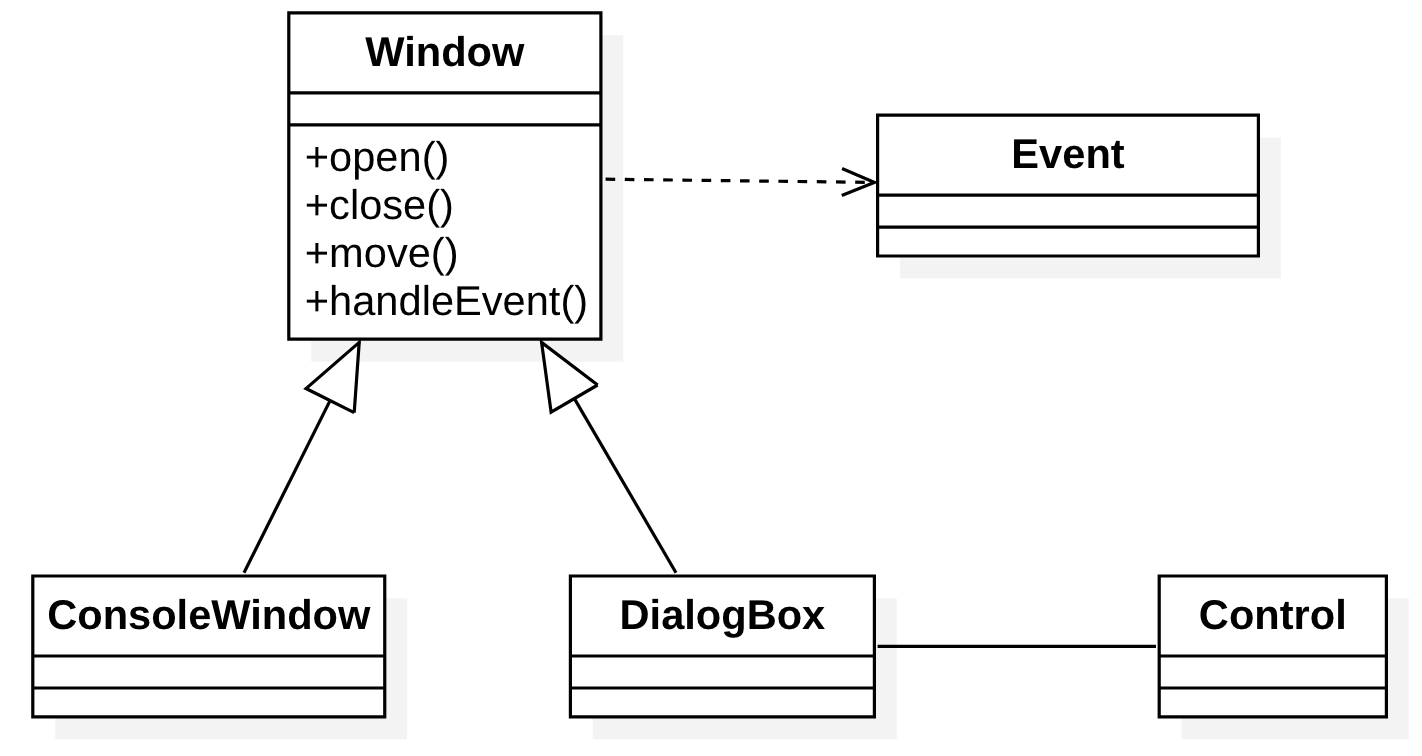
\includegraphics[scale=0.40]{ooad/uml.png}
    \end{center}

    \noindent \textbf{Klasy} składają się z \textbf{nazwy}, \textbf{atrybutów}, \textbf{operacji} i opcjonalnie
    \textbf{odpowiedzialności}.

    \begin{table}[H]
        \begin{center}
            \begin{tabular}{c}
                \textbf{Widoczność pól}\\
                \hline
                \textbf{+} public\\
                \textbf{-} private\\
                \textbf{\#} protected\\
                \textbf{\~} package
            \end{tabular}
        \end{center}
    \end{table}

    \begin{itemize}[noitemsep]
        \item \textbf{Asocjacja}

        \begin{center}
            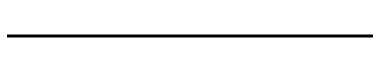
\includegraphics[scale=0.40]{ooad/association.png}
        \end{center}

        \item \textbf{Zależność} -- klasa używa innej klasy. Przykład: EventHandler i Event.
        \begin{center}
            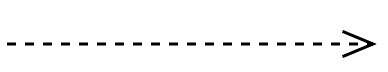
\includegraphics[scale=0.40]{ooad/dependency.png}
        \end{center}

        \item \textbf{Generalizacja} -- dziedziczenie lub uogólnienie; zależność między klasą pochodną a klasą bazową.
        \begin{center}
            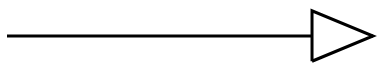
\includegraphics[scale=0.40]{ooad/generalization.png}
        \end{center}

        \item \textbf{Realizacja} -- zależność między implementacją a interfejsem. Przyład: ArrayList i List.

        \begin{center}
            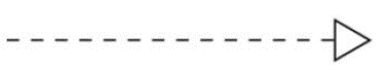
\includegraphics[scale=0.40]{ooad/realization.png}
        \end{center}

        \item \textbf{Agregacja} -- zależność między częścią a całością. Przykład: cegła i mur.

        \begin{center}
            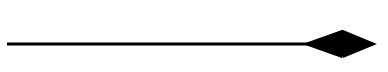
\includegraphics[scale=0.40]{ooad/composition.png}
        \end{center}

        \item \textbf{Kompozycja} (silna agregacja) -- zależność między częścią a całością, jednak część nie może
        istnieć bez całości. Przykład: wydział i uczelnia.

        \begin{center}
            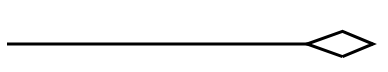
\includegraphics[scale=0.40]{ooad/aggregation.png}
        \end{center}
    \end{itemize}

    \subsection{Modele dynamiczne}

    \begin{itemize}
        \item \textbf{Diagram sekwencji} -- interakcje pomiędzy częściami systemu w postaci sekwencji
        komunikatów wymienianych między nimi; dynamiczne aspekty realizacji scenariuszy, rozdział~\ref{sec:uml}.
        \item \textbf{Diagram stanów} -- graficznareprezentacja stanów, przejść, zdarzeń i akcji maszyny stanów
        modelującej dynamiczne aspekty systemu.
    \end{itemize}

    \textbf{Diagram stanów}

    \begin{center}
        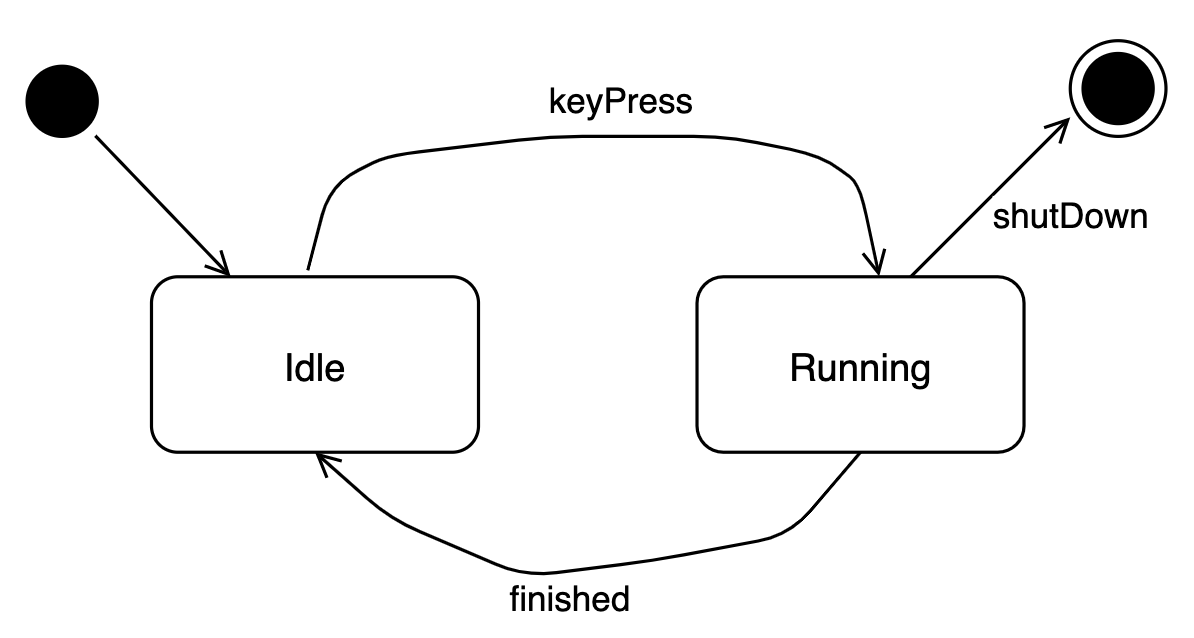
\includegraphics[scale=0.40]{state-diagram/diagram.png}
    \end{center}


    \begin{itemize}
        \item \textbf{Stan} -- sytuacja lub stan obiektu, w którym przez pewien czas spełnia on pewien warunek,
        wykonuje jakąś czynność lub czeka na jakieś zdarzenie. Wyróżniamy

        \begin{itemize}[noitemsep]
            \item Podstany -- wewnętrzne podzielenie stanu.
            \item Stan początkowy -- domyślne miejsce początkowe dla danego stanu lub automatu.
            \item Stan końcowy -- miejsce zakończenia wykonania automatu stanów.
        \end{itemize}

        \item \textbf{Przejście} -- związek między dwoma stanami wskazujący, że obiekt w pierwszym stanie wykona
        określone działania i przejdzie w drugi stan, gdy wystąpi określone zdarzenie i spełnione zostaną
        określone warunki.

        \begin{itemize}[noitemsep]
            \item Zdarzenie -- wystąpienie bodźca, który może wywołać zmianę stanu.
            \item Akcja -- wykonywalne obliczenie atomowe (np. isFinished).
        \end{itemize}
    \end{itemize}


    \subsection{Encja-Brzeg-Sterowanie}

    \textbf{Trzy} typy obiektów:
    \begin{itemize}
        \item \textbf{Obiekty brzegowe} -- odzwierciedlają interakcje między aktorami a systemem,
        \item \textbf{Obiekty sterujące} -- odpowiadają za realizację przypadków użycia,
        \item \textbf{Obiekty encji} -- reprezentujące trwałą informację przetwarzaną przez system.
    \end{itemize}
    Np. przycisk (brzegowy) $\rightarrow$ funkcjonalność zmiany daty (sterujący)  $\rightarrow$ zmiana dnia, miesiąca,
    roku (encje).


    \section{Wzorce architektury systemów.}

    \subsection{Architektura warstwowa}

    Efektem dekompozycji hierarchicznej jest \textbf{uporządkowany zbiór warstw}. Warstwa stanowi
    \textbf{zgrupowanie podsystemów} oferujących powiązane usługi.

    \noindent Zalety:
    \begin{itemize}[noitemsep]
        \item modyfikowalność
        \item prostota wykorzystania warstwy
        \item spójność i przejrzystość
        \item wielokrotne wykorzystanie
        \item naturalna ewolucja z tradycyjnego modelu aplikacji
    \end{itemize}

    \noindent \textbf{Dwa rodzaje} architektury warstwowej:
    \begin{itemize}
        \item \textbf{Architektura otwarta} -- warstwa może wywołać dowolną z warstw poniżej niej.
        Przykłady: Serverless, Swing.

        \item \textbf{Architektura zamknięta} -- warstwa może wywołać tylko wartstwę bezpośrednio pod nią.
        Przykłady: ISO/OSI, TCP/IP.
    \end{itemize}

    \noindent \textbf{Architektura trójwarstwowa} -- architektura typu klient-serwer,
    często stosowana przy tworzeniu aplikacji internetowych.
    \begin{enumerate}[noitemsep]
        \item Wartwa \textbf{prezentacji} -- interfejs użytkownika, tłumaczy żądania i wyniki.
        \item Warstwa \textbf{logiki biznesowej} -- koordynuje pracę aplikacji, przetwarza żądania
        wartstwy prezentacji, dokonuje obliczeń.
        \item Warstwa \textbf{danych} -- mechanizmy persystencji danych oraz dostępu do nich.
    \end{enumerate}

    \subsection{Model View Controller}

    Wzorzec architektoniczny, dzielący system na trzy główne części:
    \begin{enumerate}[noitemsep]
        \item \textbf{Model} reprezentuje podstawową część funkcjonalności systemu,
        \item \textbf{Widok} wyświetla dane dostarczone przez model użytkownikowi,
        \item \textbf{Kontroler} przyjmuje dane wejściowe od użytkownika oraz przetwarza jego żądania.
    \end{enumerate}

    \subsection{Pipeline (filtry i potoki)}
    \begin{itemize}[noitemsep]
        \item  Wzorzec Pipeline pozwala na \textbf{uporządkowanie systemu}, która przetwarza
        \textbf{strumienie danych}.
        \item  Każdy krok przetwarzania jest zamknięty w \textbf{filtrze}.
        \item  Dane przesyłane są pomiędzy elementami za pomocą \textbf{potoków} (pipes).
        \item Wyjście poprzedniego filtra przez potok jest przesyłane jako wejście następnego.
        \item Np. pipelnie w Unixie ($|$).
    \end{itemize}

    \subsection{Client - Server}
    \begin{itemize}[noitemsep]
        \item Podział systemu na \textbf{dostawcę} usług (server) oraz ich \textbf{odbiorców} (clients).
        \item Serwer oczekuje na żądania (request) klientów, przetwarza je, a następnie wysyła odpowiedzi (response).
        \item Serwer \textbf{pasywny}, klient \textbf{aktywny}.
        \item Przykłady: serwer WWW i przeglądarka internetowa, system bankowy.
    \end{itemize}

    \subsection{Peer-to-Peer}

    \begin{itemize}[noitemsep]
        \item \textbf{Każdy} z podsytemów (hostów, peerów) może pełnić zarówno \textbf{funkcję serwera}, jak i
        \textbf{klienta}.
        \item Architektura systemu jest rozproszona, każdy z hostów ma \textbf{te same uprawnienia}.
        \item Przykłady: torrenty, niektóre wideochaty.
    \end{itemize}

\end{document}